\par L'objectif de l'itération 1 était un prototype qui devait premièrement pouvoir se lancer et s'éteindre. De plus le prototype devait pouvoir gérer (mémorisation, affectation) des données de type chaines. Les commandes debut, defs, fin et l'instruction var ont donc été ajoutés afin d'obtenir ces fonctionnalités.

\section{Paquetage interpreteurlir.donnees.litteraux}
\begin{center}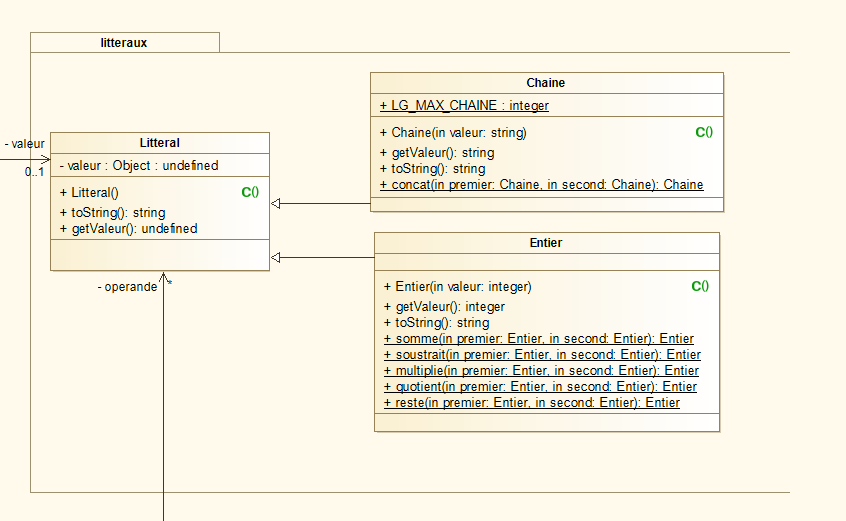
\includegraphics[scale=0.75]{./img/COO/COO_prototype_1/PackageLitteraux}\end{center}
\par Le choix de conception des littéraux a été une classe parente Litteral qui permet d'englober tous les types de données du programme.
La classe Entier a été détaillé dans la conception cependant elle n'a pas été codée à cette itération pour se concentrer sur les chaînes.
Les littéraux sont immuables pour permettre leur passage sans problème.

\section{Paquetage interpreteurlir.donnees}
\begin{center}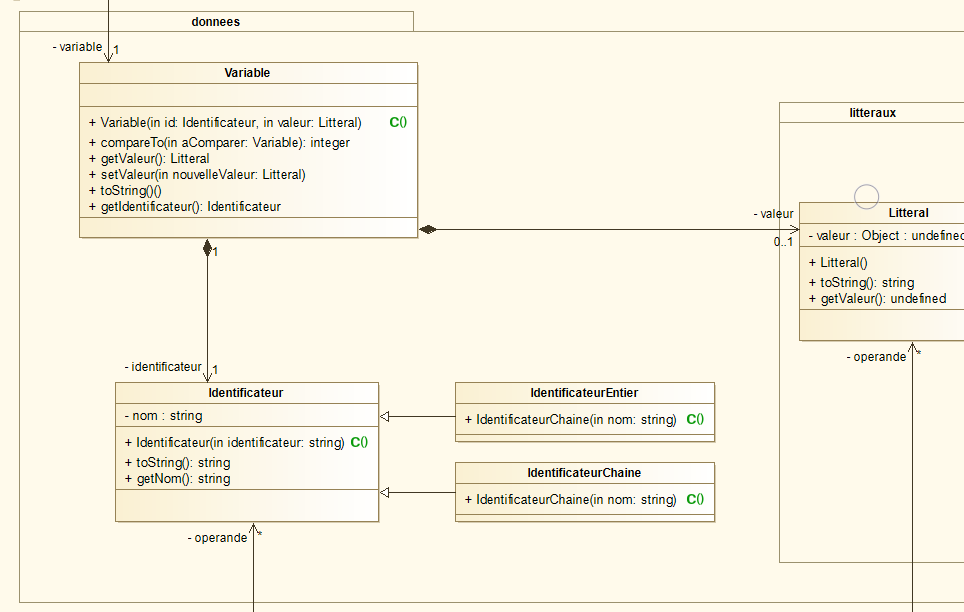
\includegraphics[scale=0.65]{./img/COO/COO_prototype_1/PackageDonnees}\end{center}
\par Pour les données une classe variable a été choisie composée d'un littéral et d'un identificateur.
L'identificateur a comme classes dérivées les deux types affectables du projet soit les entiers et les chaînes.

\section{Paquetage interpreteurlir.expressions}
\begin{center}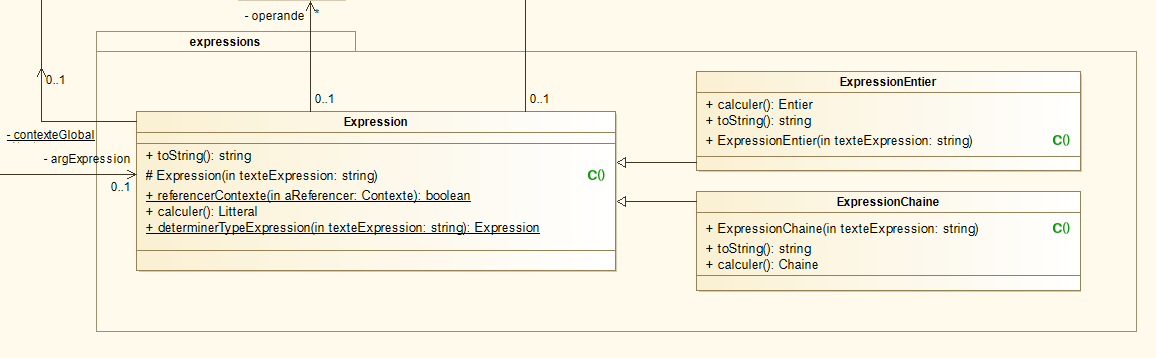
\includegraphics[scale=0.60]{./img/COO/COO_prototype_1/PackageExpressions}\end{center}
\par Comme pour le reste de notre conception les expressions sont typées et sont une spécialisation d'une classe Expression générale regroupant les comportements communs. Une méthode de classe d'Expression permet de créer le bon type d'expression.

\section{Paquetage interpreteurlir.motscles}
\begin{center}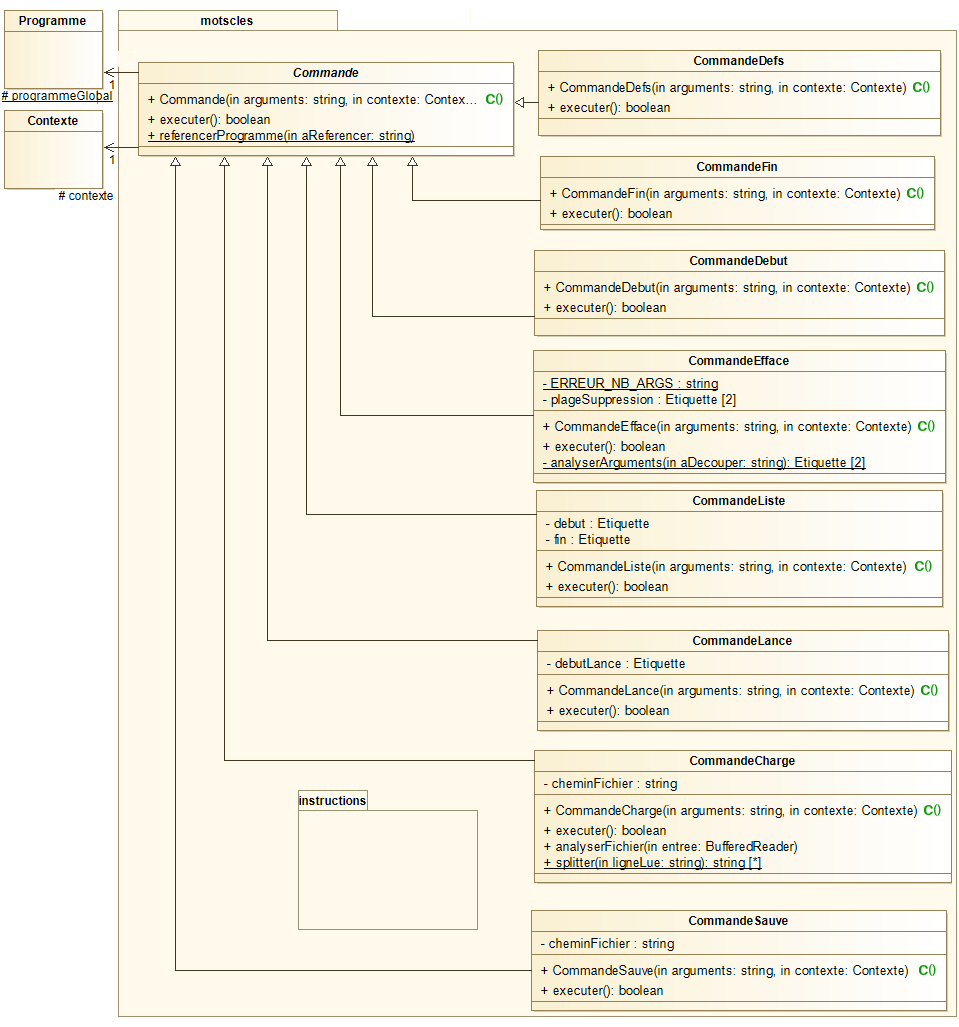
\includegraphics[scale=0.60]{./img/COO/COO_prototype_1/PackageMotscles}\end{center}
\par La conception de l'itération 1 contient ce qui devait être faits lors de cette itération à quelques détaille près comme la classe InstructionAffiche qui n'a pas été codée car non nécessaire aux fonctionnalités choisies.
L'itération 1 voulait permettre de manier des chaînes il fallait donc que les commandes connaissent le contexte contenant les variables. La solution choisie a été une attribut d'instance dans Commande initialiser à la construction de la commande par passage de la référence du contexte global par le constructeur. Une instance de commande correspond à un objet ayant toutes les informations nécessaire pour être exécuté (String arguments dans le constructeur). Les commandes et instructions fonctionnent en 2 temps, la construction qui valide les arguments et créer les éléments nécessaires à l'exécution puis l'exécution qui est la réalisation du comportement de la commande.

\section{Paquetage interpreteurlir}
\begin{center}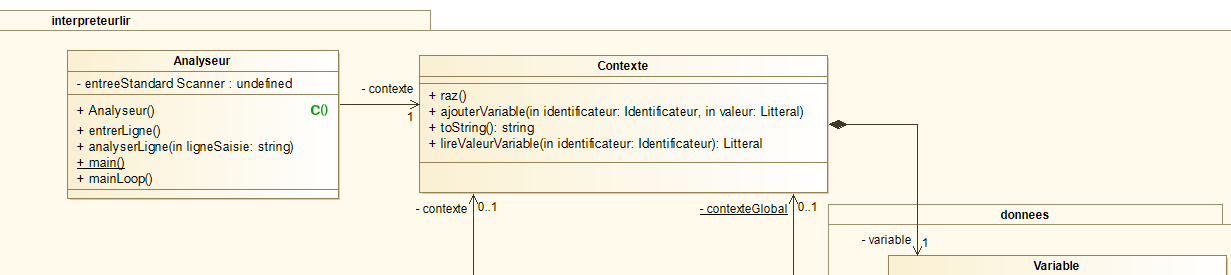
\includegraphics[scale=0.60]{./img/COO/COO_prototype_1/PackageInterpreteurlir}\end{center}
\par Le contexte regroupe l'entièreté des variables définies dans la session courante. Une variable n'est accessible que par l'intermédiaire du contexte grâce à l'identificateur qui sert de clé. L'Analyseur est la classe qui permet le fonctionnement de tout. Une mainLoop permet de demander en continue une ligne à l'utilisateur puis celle-ci est analyser, à partir du mot clé une commande/instruction est crée en passant le reste de la ligne en argument. L'analyse des arguments se fait au niveau le plus interne possible (Analyseur analyse le mot cle, la commande les arguments qui construit ensuite les éléments dont elle a besoin qui s'occupe eux-mêmes de vérifier leur validité à la construction). Si une erreur dans la ligne à interprété est détecté alors une InterpreteurException est levée et se propage jusqu'à l'analyseur qui affiche l'erreur.

\section{Illustration avec des diagrammes d'objets}
\begin{center}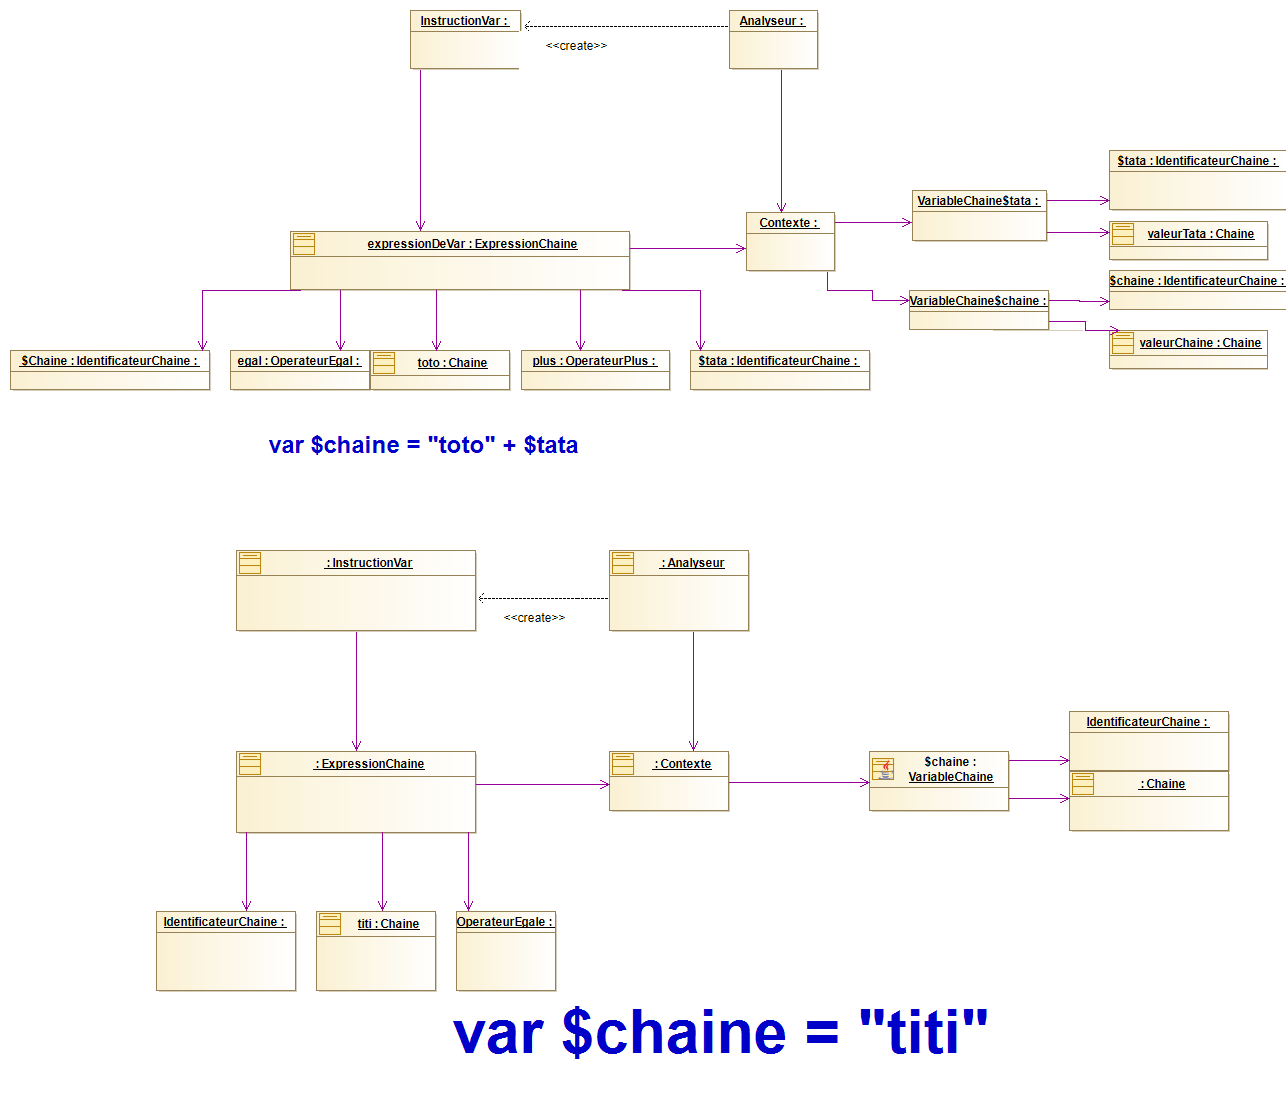
\includegraphics[scale=0.50]{./img/COO/COO_prototype_1/Objet}\end{center}
\par Voici des diagrammes qui ont été faits pendant la réflexion de cette conception. Ils permettent d'illustrer le fait qu'une instruction créer les éléments dont elle a besoin. Seul changement dans la conception par rapport à ces diagrammes : les opérateurs sont gérer en interne des instructions (il n'y pas de classe Operateur).